% #-*- coding:utf-8 -*-
\documentclass[8pt]{beamer}
\usepackage[space,noindent]{ctex}
\usepackage{beamerthemeshadow}

\title{Omega and Phi ratio}
\author{xiaohai}
\date{\today}

\begin{document}
% _______________________________________________________________
\begin{frame}
  \titlepage
\end{frame}

% _______________________________________________________________
\begin{frame}
  \frametitle{{幻灯片测试}} %\pause
  我的第一张幻灯片.
  % 定义的使用
  \begin{definition}
    definition 1...
  \end{definition}

  % theorem的使用  
  \begin{theorem}
    theorem的使用...
  \end{theorem}

  % proof的使用
  \begin{proof}
    证明
  \end{proof}

  % example的使用
  \begin{example}
    例子
  \end{example}

  % 使用\alert{内容}对内容进行强调为红色.
  % 使用\structure{内容}对内容进行强调为蓝色.
  \alert{看啥看,我是红的.}
  \structure{不用看.我是蓝的.}

\end{frame}

% _______________________________________________________________
\begin{frame}
  \frametitle{第二章幻灯片} %\pause
  \begin{itemize}
  \item beamer introduction %\pause
  \item beamer details %\pause
  \item beamer conclusions
  \end{itemize}
\end{frame}

% _______________________________________________________________
\begin{frame}
  \frametitle{第三章幻灯片的标题}

  beamer还定义了三种常规的文本块。
  \begin{itemize}
  \item 常规的block
    \begin{block}{我是常规block}
      不用看了,我是常规的block。
    \end{block}
  \item 示例exampleblock
    \begin{exampleblock}{我是举例block}
      我就是举例block,但是栗子已经被我吃了.
    \end{exampleblock}
  \item 强调alertblock
    \begin{alertblock}{我是强调block}
      强调block就是我。
    \end{alertblock}
  \end{itemize}
  
\end{frame}

% _______________________________________________________________
\begin{frame}
  \setbeamercolor{colorbox}{fg=black, bg=pink}
  \setbeamercolor{boxupper}{fg=red, bg=blue}
  \setbeamercolor{boxlower}{fg=yellow, bg=pink}
  \frametitle{文本盒子环境}
  beamer还提供了用于修饰文本的文本盒子环境:
  \begin{enumerate}
  \item 彩色盒子环境\newline
    最优美的物理公式:\newline
    \centerline{
      \begin{beamercolorbox}[rounded=true,shadow=true,wd=15mm]{colorbox}
        $E = m~c^2$
      \end{beamercolorbox}
    }
  \item 圆角盒子环境\newline
    \begin{beamerboxesrounded}[upper=boxupper, lower=boxlower,shadow=true]{标题}
      我是圆角盒子的内容。
    \end{beamerboxesrounded}
  \end{enumerate}
\end{frame}

% _______________________________________________________________
\begin{frame}
  \frametitle{列表的使用}
  列表最常用的是常规列表环境itemize和排序列表环境enumerate,
  它们可以直接在帧环境中使用,也可以置于block环境中。
  \begin{block}{我对tex的印象}

    \begin{enumerate}
    \item 我靠,这东西做出来的PDF怎么能这么漂亮!
    \item Fuck,这东西怎么这么难学。
    \item 额,原来学这东西也是有方法的啊。
    \end{enumerate}

  \end{block}
\end{frame}

% _______________________________________________________________

\begin{frame}
  \frametitle{columns}
  \texttt{columns}我们可以将一页分成多栏,通常左栏为图,又栏为文字。
  \begin{columns}[onlytextwidth]
    \begin{column}{0.55\textwidth}
      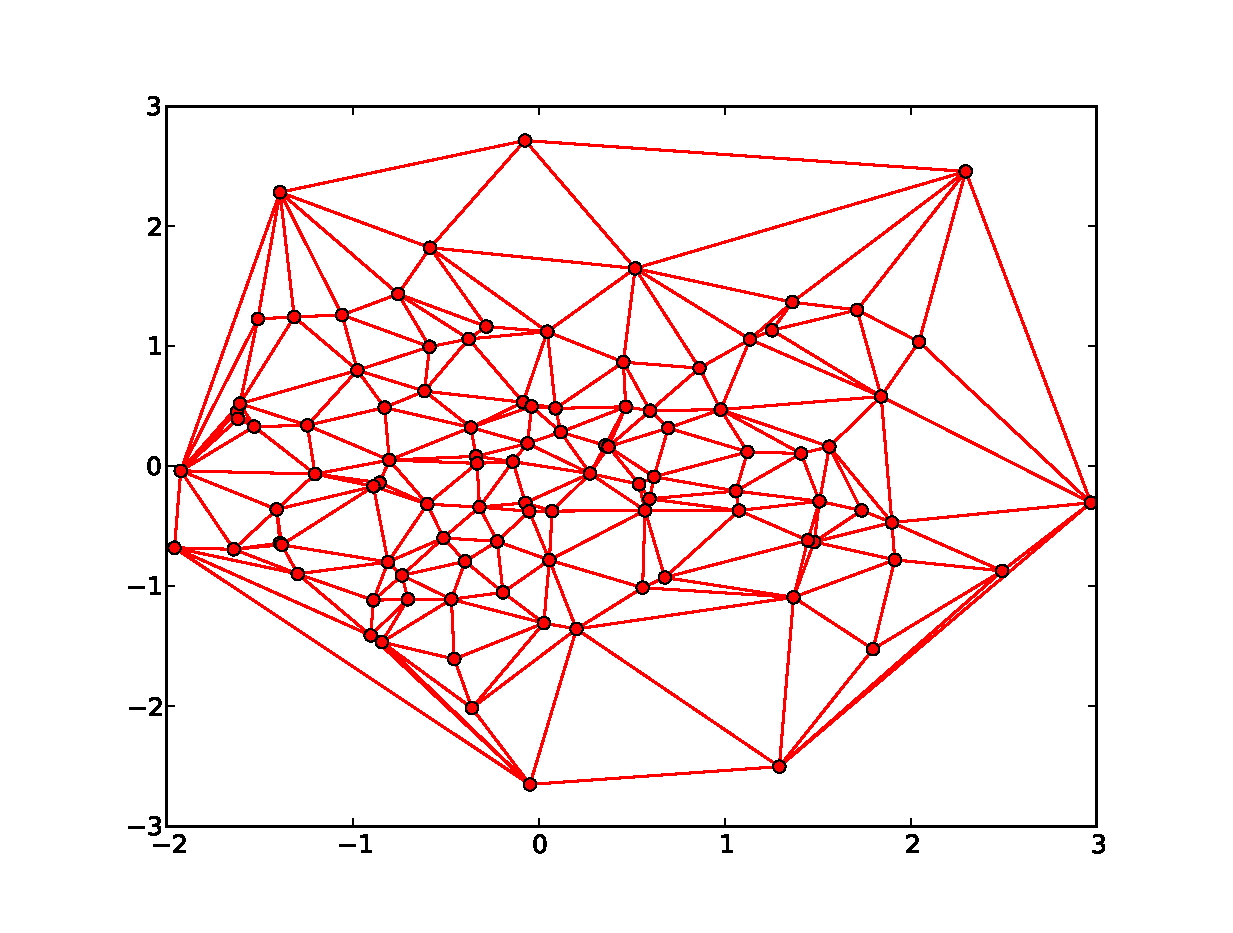
\includegraphics[width=\columnwidth]{./triangle.eps}
    \end{column}
    \begin{column}{0.45\textwidth}
      左图是我用matplotlib做出来的。
      \begin{enumerate}
      \item matplotlib是一个很好的做图库。
      \item 该软件库也很容易学习。
      \item 更关键的是做出来的图亮瞎眼。
      \end{enumerate}
    \end{column}
  \end{columns}
\end{frame}

% _______________________________________________________________
\begin{frame}
  \frametitle{参考文献}
  \begin{thebibliography}{99}
  \beamertemplatetextbibitems
  \bibitem{xiaohai} 自己去歪歪吧
  \end{thebibliography}
\end{frame}

\end{document}

%%% Local Variables:
%%% mode: latex
%%% TeX-master: t
%%% End:

